\documentclass[notitlepage,aps,prd,nofootinbib]{revtex4-1}

\usepackage{subfig}
%\usepackage[colorinlistoftodos]{todonotes}
\usepackage{float}

%\usepackage[protrusion=true,expansion=true]{microtype}
\usepackage{amsmath}
\usepackage{amssymb}
\usepackage{bbm}
\usepackage{ulem}
%\usepackage{feynmp-auto}
%\usepackage{slashed}
%\usepackage[absolute,overlay]{textpos}
\usepackage[usenames, dvipsnames]{color}
\usepackage{graphicx}
\usepackage{listings}
\usepackage{epsfig}
\usepackage{hyperref}
%\usepackage{tikz}
\usepackage{enumerate}
%\usepackage{fixltx2e} % buggy
\usepackage[compatibility=false]{caption}
%\usepackage{subcaption} % doesn't work with subfigure
\usepackage{pdfpages}
%\usepackage{setspace}
\usepackage{verbatim}

% Turn off meaningless float warnings
\usepackage{silence}
\WarningFilter{revtex4-1}{Repair the float}

\DeclareRobustCommand{\orderof}{\ensuremath{\mathcal{O}}}

\definecolor{dukeblue}{RGB}{0,0,156}
\definecolor{dukedarkblue}{RGB}{0,26,87}
\definecolor{dukeblack}{RGB}{79,79,79}
\definecolor{dukegray}{RGB}{79,79,79}
\definecolor{dukesecbrown}{RGB}{217,200,158}
\definecolor{dukesecblue}{RGB}{127,169,174}

%\renewcommand*{\thefootnote}{\fnsymbol{footnote}}

%%%%%%%%%%%%%%%%%%%%%%%%%%%%%%%%%%%%%%%%%%%%%%%%%%%%%%%%%%%%%%%%%%%%%%%%%%%%%%%%%%%%%
\hypersetup{
    breaklinks,
    baseurl       = http://,
    pdfborder     = 0 0 0,
    pdfpagemode   = UseNone,% do not show thumbnails or bookmarks on opening
    pdfstartpage  = 1,
    bookmarksopen = true,
    bookmarksdepth= 2,% to show sections and subsections
% revtex needs author and title declared after \begin{document}, so have to hard code them...
%    pdfauthor     = {\@author},
%    pdftitle      = {\@title},
    pdfauthor     = {Matthew Epland},
    pdftitle      = {Phys 566 Midterm},
    pdfsubject    = {},
    pdfkeywords   = {}}


% Code import settings
%%%%%%%%%%%%%%%%%%%%%%%%%%%%%%%%%%%%%%%%%%%%%%%%%%%%%%%%%%%%%%%%%%%%%%%%%%%%%%%%%%%%%
\definecolor{mygreen}{rgb}{0,0.6,0}
\definecolor{mygray}{rgb}{0.5,0.5,0.5}
\definecolor{mymauve}{rgb}{0.58,0,0.82}

%\lstset{ %
\lstdefinestyle{python}{ %
  backgroundcolor=\color{white},   % choose the background color; you must add \usepackage{color} or \usepackage{xcolor}
  basicstyle=\scriptsize,          % the size of the fonts that are used for the code
  breakatwhitespace=false,         % sets if automatic breaks should only happen at whitespace
  breaklines=true,                 % sets automatic line breaking
  captionpos=b,                    % sets the caption-position to bottom
  commentstyle=\color{mygreen},    % comment style
  deletekeywords={...},            % if you want to delete keywords from the given language
  escapeinside={\%*}{*)},          % if you want to add LaTeX within your code
  extendedchars=true,              % lets you use non-ASCII characters; for 8-bits encodings only, does not work with UTF-8
  frame=single,	                   % adds a frame around the code
  keepspaces=true,                 % keeps spaces in text, useful for keeping indentation of code (possibly needs columns=flexible)
  keywordstyle=\color{blue},       % keyword style
  language=Python,                 % the language of the code
  otherkeywords={*,...},           % if you want to add more keywords to the set
  numbers=left,                    % where to put the line-numbers; possible values are (none, left, right)
  numbersep=5pt,                   % how far the line-numbers are from the code
  numberstyle=\tiny\color{mygray}, % the style that is used for the line-numbers
  rulecolor=\color{black},         % if not set, the frame-color may be changed on line-breaks within not-black text (e.g. comments (green here))
  showspaces=false,                % show spaces everywhere adding particular underscores; it overrides 'showstringspaces'
  showstringspaces=false,          % underline spaces within strings only
  showtabs=false,                  % show tabs within strings adding particular underscores
  stepnumber=5,                    % the step between two line-numbers. If it's 1, each line will be numbered
  stringstyle=\color{mymauve},     % string literal style
  tabsize=2,	                   % sets default tabsize to 2 spaces
%  title=\lstname                   % show the filename of files included with \lstinputlisting; also try caption instead of title
  title={\protect\filename@parse{\lstname}\protect\filename@base.\filename@ext},
  firstnumber=0,
%  linewidth=0.95\textwidth
  xleftmargin=0.01\textwidth,
  xrightmargin=0.01\textwidth
}

\lstdefinestyle{output}{ %
  backgroundcolor=\color{white},   % choose the background color; you must add \usepackage{color} or \usepackage{xcolor}
  basicstyle=\scriptsize,          % the size of the fonts that are used for the code
  breakatwhitespace=false,         % sets if automatic breaks should only happen at whitespace
  breaklines=true,                 % sets automatic line breaking
  captionpos=b,                    % sets the caption-position to bottom
  escapeinside={\%*}{*)},          % if you want to add LaTeX within your code
  frame=single,	                   % adds a frame around the code
  keepspaces=true,                 % keeps spaces in text, useful for keeping indentation of code (possibly needs columns=flexible)
  numbers=left,                    % where to put the line-numbers; possible values are (none, left, right)
  numbersep=5pt,                   % how far the line-numbers are from the code
  numberstyle=\tiny\color{mygray}, % the style that is used for the line-numbers
  rulecolor=\color{black},         % if not set, the frame-color may be changed on line-breaks within not-black text (e.g. comments (green here))
  stepnumber=5,                    % the step between two line-numbers. If it's 1, each line will be numbered
  tabsize=2,	                   % sets default tabsize to 2 spaces
%  title=\lstname                   % show the filename of files included with \lstinputlisting; also try caption instead of title
  title={\protect\filename@parse{\lstname}\protect\filename@base.\filename@ext},
  firstnumber=0,
%  linewidth=0.95\textwidth
  xleftmargin=0.01\textwidth,
  xrightmargin=0.01\textwidth
}

\newcommand{\degree}{\ensuremath{^{\circ}}}

% TODO Select between raw and saved plots here
\graphicspath{{../code/output/plots_for_paper/}} % raw plots
%\graphicspath{{./output/}} % saved plots

%%%%%%%%%%%%%%%%%%%%%%%%%%%%%%%%%%%%%%%%%%%%%%%%%%%%%%%%%%%%%%%%%%%%%%%%%%%%%%%%%%%%%
\begin{document}

\title{PHYS 566 Midterm}
\author{Matthew Epland}
\affiliation{Department of Physics, Duke University, Durham, NC 27707, USA}

\date{\today}

\begin{abstract}
TODO
\end{abstract}\maketitle


\section{Introduction}
\label{sec:intro}
TODO

\section{Theory}
\label{sec:theory}
TODO


\begin{equation} \label{eq:jacobi}
V_{\mathrm{new}}\left(i,j\right)^{\mathrm{Jacobi}} = \frac{1}{2^2}\big( V_{\mathrm{old}}\left(i+1,j) + V_{\mathrm{old}}\left(i-1,j) +V_{\mathrm{old}}\left(i,j+1) +V_{\mathrm{old}}\left(i,j-1) \big)
\end{equation}

\begin{equation} \label{eq:GS}
V_{\mathrm{new}}\left(i,j\right)^{\mathrm{GS}} = \frac{1}{2^2}\big( V_{\mathrm{latest}}\left(i+1,j) + V_{\mathrm{latest}}\left(i-1,j) +V_{\mathrm{latest}}\left(i,j+1) +V_{\mathrm{latest}}\left(i,j-1) \big)
\end{equation}

\begin{comment
\begin{align} \label{eq:SOR}
V_{\mathrm{new}}\left(i,j\right)^{\mathrm{SOR}} = V\left(i,j\right)^{\mathrm{GS}} - V\left(i,j\right)^{\mathrm{GS}} 

\end{equation}
\end{comment}

\clearpage
\section{Results}
\label{sec:results}
TODO


\clearpage
\subsection{Part 1.A}
\label{subsec:part_1a}

\begin{figure}[!htbc]
  \centering
  \includegraphics[width=.7\textwidth]{poisson_dipole/part_a/V_best_jacobi.pdf}
	{\par\nobreak\rule[9pt]{35em}{0.5pt}\vspace{-5mm}}
	\caption{$V\left(x, y\right)$, Jacobi method.}
	\label{fig:part1a_V}
\end{figure}

\clearpage
\begin{figure}[!htbc]
  \centering
  \includegraphics[width=.7\textwidth]{poisson_dipole/part_a/Vr_dipole_axis_best_jacobi.pdf}
	{\par\nobreak\rule[9pt]{35em}{0.5pt}\vspace{-5mm}}
	\caption{$V\left(r, \theta=0\right)$, through the dipole's axis, Jacobi method.}
	\label{fig:part1a_Vr}
\end{figure}

\clearpage
\subsection{Part 1.B}
\label{subsec:part_1b}

% TODO
\begin{comment}
\begin{figure}[!htbc]
  \centering
  \includegraphics[width=.7\textwidth]{poisson_dipole/part_b/
	{\par\nobreak\rule[9pt]{35em}{0.5pt}\vspace{-5mm}}
	\caption{$N_{\mathrm{iter}}\left(\epsilon\right)$, Jacobi method}
	\label{fig:part1b}
\end{figure}
\end{comment}

\clearpage
\subsection{Part 1.C}
\label{subsec:part_1c}

% TODO
\begin{comment}
\begin{figure}[!htbc]
  \centering
  \includegraphics[width=.7\textwidth]{poisson_dipole/part_c/
	{\par\nobreak\rule[9pt]{35em}{0.5pt}\vspace{-5mm}}
	\caption{$N_{\mathrm{iter}}\left(n\right)$, Jacobi and SOR methods with absolute convergence, $A <$ 0.001.}
	\label{fig:part1b}
\end{figure}
\end{comment}

\clearpage
\subsection{Part 2.A}
\label{subsec:part_2a}

\begin{figure}[!htbc]
  \centering
  \includegraphics[width=.7\textwidth]{biot_savart/part_a_Bxyz_of_z.pdf}
	{\par\nobreak\rule[9pt]{35em}{0.5pt}\vspace{-5mm}}
	\caption{$\mathbf{B}\left(x=y=0,~z\right)$ with the theoretical result for a similar circular current loop.}
	\label{fig:part2a}
\end{figure}

\clearpage
\subsection{Part 2.B}
\label{subsec:part_2b}

\begin{figure}[!htbc]
  \centering
  \includegraphics[width=.6\textwidth]{biot_savart/part_b_Bxyz_of_x.pdf}
	{\par\nobreak\rule[9pt]{35em}{0.5pt}\vspace{-5mm}}
	\caption{$\mathbf{B}\left(y=0,~z=1\mathrm{m},~x\right)$}
	\label{fig:part2b}
\end{figure}

\subsection{Part 2.C}
\label{subsec:part_2c}

\begin{figure}[!htbc]
  \centering
  \includegraphics[width=.6\textwidth]{biot_savart/part_c_Bxyz_of_z.pdf}
	{\par\nobreak\rule[9pt]{35em}{0.5pt}\vspace{-5mm}}
	\caption{$\mathbf{B}\left(x=0.5\mathrm{m},~y=0,~z\right)$}
	\label{fig:part2c}
\end{figure}


\clearpage
\section{Conclusions}
\label{sec:Conclusions}
TODO

The Python source code used to produce these results can be found online at \url{http://github.com/mepland/PHYS_566_Computational_HW/tree/master/midterm/code}, and is included in Section~\ref{sec:code}.

\clearpage
\section{Extra Material}
\label{sec:Extra_Material}

\begin{figure}[!htbc]
  \centering
  \includegraphics[width=.7\textwidth]{poisson_dipole/extra_material/V_boundary_best_jacobi.pdf}
	{\par\nobreak\rule[9pt]{35em}{0.5pt}\vspace{-5mm}}
	\caption{Boundary conditions diagnostic test.}
	\label{fig:boundary_test}
\end{figure}

\begin{figure}[!htbc]
  \centering
  \includegraphics[width=.7\textwidth]{poisson_dipole/extra_material/V_initial_best_jacobi.pdf}
	{\par\nobreak\rule[9pt]{35em}{0.5pt}\vspace{-5mm}}
	\caption{Initial array diagnostic test.}
	\label{fig:initial_array_test}
\end{figure}

\begin{comment}
TODO
\clearpage
\begin{figure}[!htbc]
  \centering
  \includegraphics[width=.7\textwidth]{poisson_dipole/extra_material/
	{\par\nobreak\rule[9pt]{35em}{0.5pt}\vspace{-5mm}}
	\caption{If the convergence criteria are too loose, $N_{\mathrm{iter}}$ may not be large enough for the information/charge close to the origin to propagate via the average of nearest neighbors through the whole simulated region. A forced $N_{\mathrm{iter}}$ minimum would solve this potential issue, but would also complicate the $N_{\mathrm{iter}}\left(\epsilon\right)$ and $N_{\mathrm{iter}}\left(n\right)$ results.}
	\label{fig:propegation_test}
\end{figure}
\end{comment}

\clearpage
\section{Supporting Material}
\label{sec:Supporting_Material}

% TODO
% \lstinputlisting[style=output,label={lst:output}]{../code/output/output.log} % raw

\clearpage
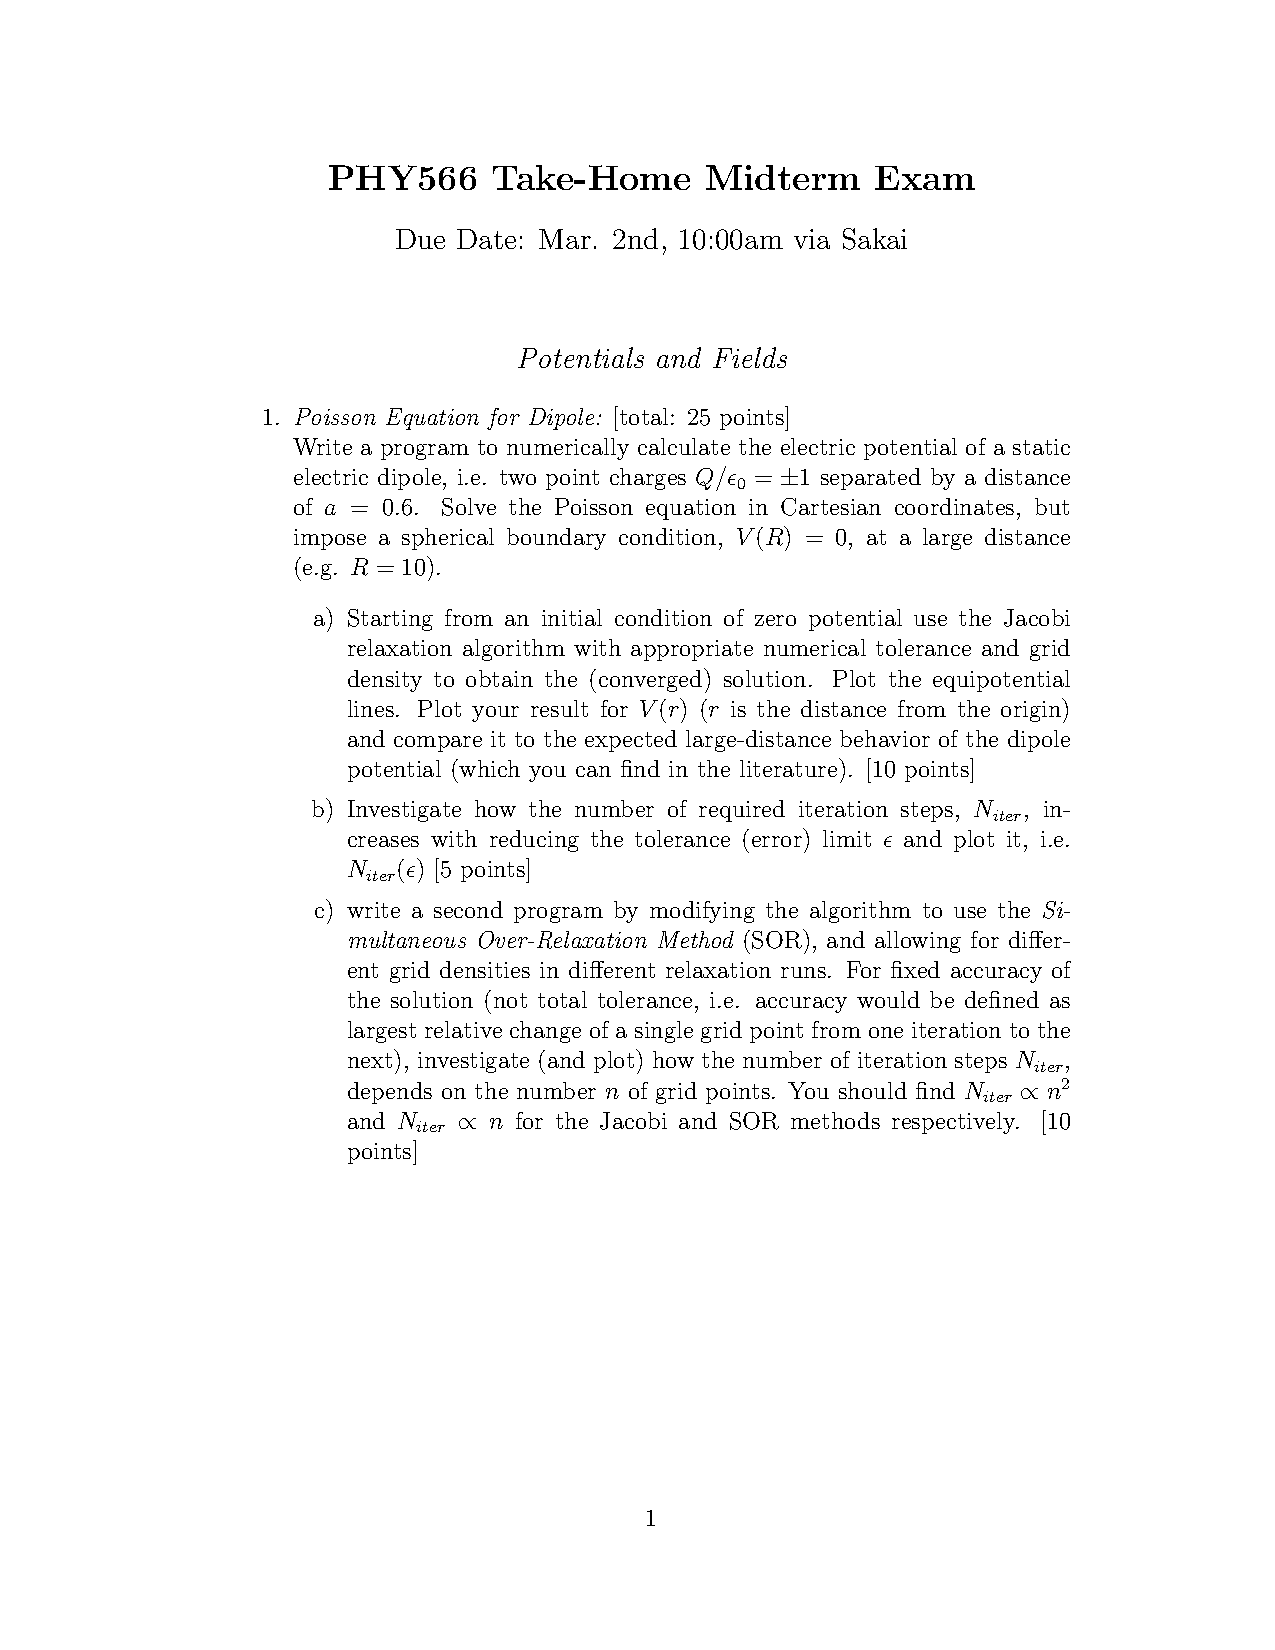
\includepdf[pages={1}]{../midterm.pdf}
\clearpage
\includepdf[pages={2}]{../midterm.pdf}
% Have to do them one a time for some reason or they overlap...

\clearpage
\section{Code}
\label{sec:code}

% TODO
% \lstinputlisting[style=python]{../code/poisson_dipole.py}
% \lstinputlisting[style=python]{../code/biot_savart.py}

\end{document} %%% end of doc %%%
%%%%%%%%%%%%%%%%%%%%%%%%%%%%%%%%%%%%%%%%%%%%%%%%%%%%%


\bibliographystyle{bib_files/styles/atlasBibStyleWoTitle}
\bibliography{bib_files/my_bib.bib}

\begin{figure}[!htbc]
  \centering
  \includegraphics[width=.6\textwidth]{part_b/compare_runs_vary_sim_method/theta_vary_sim_method.pdf}
	{\par\nobreak\rule[9pt]{35em}{0.5pt}\vspace{-5mm}}
	\caption{$\theta\left(t\right)$ for the Euler--Cromer and RK4 methods.}
	\label{fig:theta_vary_sim_method}
\end{figure}

